\documentclass[UTF8, a4paper, 11pt]{article}
\usepackage[UTF8, scheme=plain]{ctex}
\usepackage{fontspec}
\usepackage{float}
\usepackage{amsmath}
\newtheorem{myDef}{Definition}
\usepackage{graphicx}
\usepackage{geometry}
\usepackage{listings}
\usepackage{xcolor}
\usepackage{caption,subcaption}
\geometry{scale=0.8}
\linespread{1.5}
\usepackage{hyperref}
\usepackage{color}
\usepackage{fontspec}
\usepackage{enumitem}
\usepackage[linesnumbered,boxed]{algorithm2e}    
\usepackage{xeCJK}
\usepackage{indentfirst} 
\graphicspath{{Pic/}} 	% 在于.tex同级的目录下创建名为pic的文件夹,存放图片


\setlength{\parindent}{2em}

\lstset{
    language={C++},
    frame=shadowbox,
    breaklines=true,
    numbers=left,
    backgroundcolor=\color[RGB]{245,245,244},
    rulesepcolor=\color{red!20!green!20!blue!20},
    numberstyle={\color[RGB]{0,192,192}\tiny},
    basicstyle=\footnotesize \fontspec{Source Code Pro}
}
\setenumerate[1]{itemsep=0pt,partopsep=0pt,parsep=\parskip,topsep=0pt}
\setitemize[1]{itemsep=0pt,partopsep=0pt,parsep=\parskip,topsep=0pt}
\setdescription{itemsep=0pt,partopsep=0pt,parsep=\parskip,topsep=0pt}


\title{	
\normalfont \normalsize
\textsc{School of Data and Computer Science, Sun Yat-sen University} \\ [25pt] %textsc small capital letters
\rule{\textwidth}{0.5pt} \\[0.4cm] % Thin top horizontal rule
\huge CUDA和BVH\\ % The assignment title
\rule{\textwidth}{2pt} \\[0.5cm] % Thick bottom horizontal rule
\author{18308045 Zhengyang Gu}
\date{\normalsize\today}
}

\begin{document}
\maketitle
\tableofcontents
\newpage
\section{Abstract}
基础版本的光线追踪的大致流程是:将图像的每个像素视作射入摄像头的每一束光线,串行地计算每个射入光线的颜色;计算射入光线时需要遍历全部的物体以获得光线最近接触物体的一些信息来进行后续
计算。这两个点就分别是CUDA和BVH所要优化的地方。
\section{CUDA}
由于每个射入光线是没有依赖关系的,所以理想情况下可以对每个射入光线并行计算。在这里我用CUDA来实现射入光线间的并行。
\subsection{实现要点}
\subsubsection{写图像}
写图像对每个像素点是有顺序要求的,要求从左上角一行行写到右下角。而最初的实现是将计算射入光线颜色和写像素点两个步骤合在一起的,即每算完一个射入光线就会写一个像素点:
\begin{lstlisting}
// Render

std::cout << "P3\n" << image_width << " " << image_height << "\n255\n";

for (int j = image_height-1; j >= 0; --j) {
    std::cerr << "\rScanlines remaining: " << j << ' ' << std::flush;
    for (int i = 0; i < image_width; ++i) {
        color pixel_color(0, 0, 0);
        for (int s = 0; s < samples_per_pixel; ++s) {
            auto u = (i + random_double()) / (image_width-1);
            auto v = (j + random_double()) / (image_height-1);
            ray r = cam.get_ray(u, v);
            pixel_color += ray_color(r, world, max_depth);
        }
        write_color(std::cout, pixel_color, samples_per_pixel);
    }
}
\end{lstlisting}
write\_color即是将像素点写入流。这样不利于并行。这里我将这两个步骤分开操作,先并行地算完所有像素点的颜色,再串行地写入图像:
\begin{lstlisting}
// Output FB as Image
std::cout << "P3\n" << image_width << ' ' << image_height << "\n255\n";
for (int j = image_height - 1; j >= 0; j--) {
    for (int i = 0; i < image_width; i++) {
        size_t pixel_index = j * 3 * image_width + i * 3;
        std::cout << fb[pixel_index + 0] << ' ' << fb[pixel_index + 1] << ' ' << fb[pixel_index + 2] << '\n';
    }
}
\end{lstlisting}
其中fb是已经算好的全部像素点的RGB。
\subsubsection{浮点数精度}
原先的实现中浮点数精度默认是双精度,如:
\begin{lstlisting}
// Constants

const double infinity = std::numeric_limits<double>::infinity();
const double pi = 3.1415926535897932385;

// Utility Functions

inline double degrees_to_radians(double degrees) {
    return degrees * pi / 180.0;
}
\end{lstlisting}
其中有显性的双精度double和隐性的双精度180.0。而现在的GPU在双精度的计算上比单精度慢数倍,因而为了进一步提速,将所有的双精度都改成单精度:
\begin{lstlisting}
// Constants

__device__ float infinity = std::numeric_limits<float>::infinity();
__device__ float pi = 3.1415926535897932385f;

// Utility Functions

__device__ inline float degrees_to_radians(float degrees) {
    return degrees * pi / 180.0f;
}
\end{lstlisting}
\subsubsection{STL的数据结构}
原先的实现运用了很多STL的数据结构如vector,shared\_ptr:
\begin{lstlisting}
class hittable_list : public hittable {
    public:
        hittable_list() {}
        hittable_list(shared_ptr<hittable> object) { add(object); }

        void clear() { objects.clear(); }
        void add(shared_ptr<hittable> object) { objects.push_back(object); }

        virtual bool hit(
            const ray& r, double t_min, double t_max, hit_record& rec) const override;

    public:
        std::vector<shared_ptr<hittable>> objects;
};
\end{lstlisting}
而由于STL的数据结构是基于内存而非显存实现的,无法被GPU利用。所以在这里都改成普通的指针:
\begin{lstlisting}
class hittable_list : public hittable {
    public:
        __device__ hittable_list() {}
        __device__ hittable_list(hittable** list, size_t len) : objects(list), size(len) { }
        __device__ virtual bool hit(
            const ray& r, float t_min, float t_max, hit_record& rec) const override;
        __device__ virtual bool bounding_box(
            float time0, float time1, aabb& output_box) const override;

    public:
        hittable** objects;
        size_t size;
};
\end{lstlisting}
\subsubsection{随机数}
在原本的实现中诸多地方用到了随机数,如去锯齿、求漫反射模拟摄像头的光圈等等,这些随机数都用到了cstdlib的随机数实现:
\begin{lstlisting}
#include <cstdlib>
...

inline double random_double() {
    // Returns a random real in [0,1).
    return rand() / (RAND_MAX + 1.0);
}
\end{lstlisting}
而这个库是host的函数不能被device调用。在device函数中的随机数,需要用curand\_kernel.h库的实现:
\begin{lstlisting}
#include <curand_kernel.h>
...

__device__ inline float random_float(curandState* local_rand_state) {
    // Returns a random real in [0,1).
    return curand_uniform(local_rand_state);
}
\end{lstlisting}
而在计算机上的随机数实现实际上是通过伪随机数的实现,因而需要记录GPU上每个线程的状态,这就需要开设并初始化一个rand\_state空间:
\begin{lstlisting}
__global__ void random_init(int image_width, int image_height, curandState* rand_state) {
	int i = threadIdx.x + blockIdx.x * blockDim.x;
	int j = threadIdx.y + blockIdx.y * blockDim.y;
	if ((i >= image_width) || (j >= image_height)) return;
	int pixel_index = j * image_width + i;
	//Each thread gets same seed, a different sequence number, no offset
	curand_init(1984, pixel_index, 0, &rand_state[pixel_index]);
}
\end{lstlisting}
\subsubsection{数学函数}
原先实现运用到的一些数学函数是来自cmath库的:
\begin{lstlisting}
#include <cmath>
...

vec3 refract(const vec3& uv, const vec3& n, double etai_over_etat) {
    auto cos_theta = fmin(dot(-uv, n), 1.0);
    vec3 r_out_perp =  etai_over_etat * (uv + cos_theta*n);
    vec3 r_out_parallel = -sqrt(fabs(1.0 - r_out_perp.length_squared())) * n;
    return r_out_perp + r_out_parallel;
}
\end{lstlisting}
而这些函数同样是host函数,没法被device函数调用,所以这里单独建了个math.h头文件来自己实现一些用得到的数学函数:
\begin{lstlisting}
#ifndef MATH_H
#define MATH_H

__device__ inline float fmin(float& a, float& b)
{
    return a <= b ? a : b;
}

__device__ inline float fmax(float& a, float& b)
{
    return a >= b ? a : b;
}

__device__ inline float fabs(float& a)
{
    return a >= 0 ? a : -a;
}

#endif
\end{lstlisting}
\subsubsection{尾递归优化}
原先实现中计算光线颜色的地方用到了不必要的尾递归:
\begin{lstlisting}
color ray_color(const ray& r, const hittable& world, int depth) {
    hit_record rec;

    // If we've exceeded the ray bounce limit, no more light is gathered.
    if (depth <= 0)
        return color(0,0,0);

    if (world.hit(r, 0.001, infinity, rec)) {
        ray scattered;
        color attenuation;
        if (rec.mat_ptr->scatter(r, rec, attenuation, scattered))
            return attenuation * ray_color(scattered, world, depth-1);
        return color(0,0,0);
    }

    vec3 unit_direction = unit_vector(r.direction());
    auto t = 0.5*(unit_direction.y() + 1.0);
    return (1.0-t)*color(1.0, 1.0, 1.0) + t*color(0.5, 0.7, 1.0);
}
\end{lstlisting}
这可能会浪费栈内存导致栈溢出,因而改成循环:
\begin{lstlisting}
__device__ color ray_color(const ray& r, hittable_list** world, int max_depth, curandState *local_rand_state) {
    ray cur_ray = r;
	color cur_attenuation = vec3(1.0f, 1.0f, 1.0f);
    for(int i = 0; i < max_depth; i++) {
        hit_record rec;
        if ((*world)->hit(cur_ray, 0.001f, infinity, rec)) {
			ray scattered;
			color attenuation;
			if (rec.mat_ptr->scatter(cur_ray, rec, attenuation, scattered, local_rand_state))
			{
				cur_attenuation = cur_attenuation * attenuation;
				cur_ray = scattered;
			}
			else
				return color(0,0,0);
        }
        else {
            vec3 unit_direction = unit_vector(cur_ray.direction());
			float t = 0.5f * (unit_direction.y() + 1.0f);
			vec3 c = (1.0f - t) * vec3(1.0f, 1.0f, 1.0f) + t * vec3(0.5, 0.7f, 1.0f);
            return cur_attenuation * c;
        }
    }
	return vec3(0.0f, 0.0f, 0.0f); // exceeded recursion
}
\end{lstlisting}
\subsection{实验}
该部分实验基于Ray Tracing In One Weekend的最终场景,尝试了几组block的形状,每组分别测三次运行时间,并测一次原先CPU实现的运行时间作为对照。
\subsubsection{场景设置}
参数设置如下:
\begin{figure}[H]
    \centering
    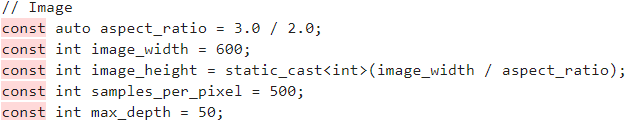
\includegraphics[width=0.8\textwidth]{hyper.png}
\end{figure}
并将场景中的小球,只保留了4个大球。
\subsubsection{block形状确定}
CUDA的device实际在执行的时候,会以Block为单位,把一个个的block分配给SM进行运算;而block中的thread,又会以「warp」为单位,把thread来做分组计算。目前CUDA的warp大小都是32,也就是32
个thread会被群组成一个warp来一起执行。在Compute Capability 1.0/1.1中,每个SM最多可以同时管理768个thread(768 active threads)或8个block(8 active blocks)。为了让工作均衡,
这就要求了:
\begin{itemize}
    \item 每个block大小是32的倍数,这样不同warp大小一致。
    \item block的宽和高要分别整除图像的宽和高,这样不同block形状类似。
\end{itemize}
由于image\_width=600,image\_height=400,我选择了块宽和块高:4x8,8x8,8x16,10x16,24x16,24x20。
\subsubsection{结果}
\begin{figure}[H]
    \centering
    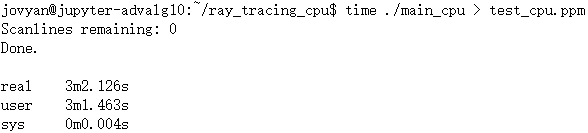
\includegraphics[width=0.8\textwidth]{cpu.png}
    \caption{CPU}
\end{figure}
\begin{figure}[H]
    \centering
    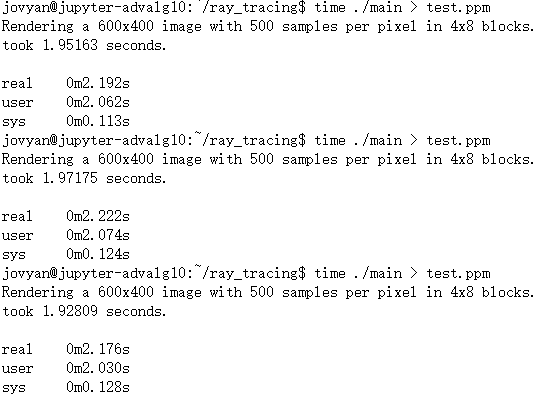
\includegraphics[width=0.8\textwidth]{4x8.png}
    \caption{CUDA with block shape 4x8}
\end{figure}
\begin{figure}[H]
    \centering
    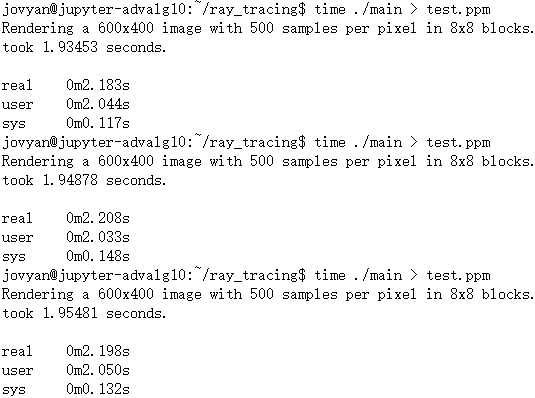
\includegraphics[width=0.8\textwidth]{8x8.png}
    \caption{CUDA with block shape 8x8}
\end{figure}
\begin{figure}[H]
    \centering
    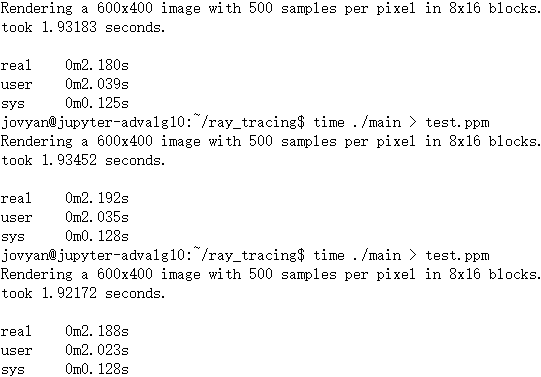
\includegraphics[width=0.8\textwidth]{8x16.png}
    \caption{CUDA with block shape 8x16}
\end{figure}
\begin{figure}[H]
    \centering
    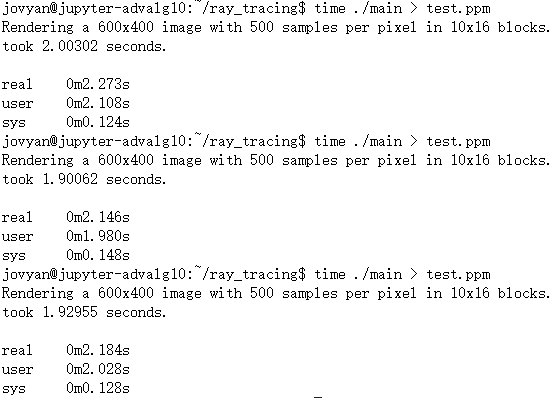
\includegraphics[width=0.8\textwidth]{10x16.png}
    \caption{CUDA with block shape 10x16}
\end{figure}
\begin{figure}[H]
    \centering
    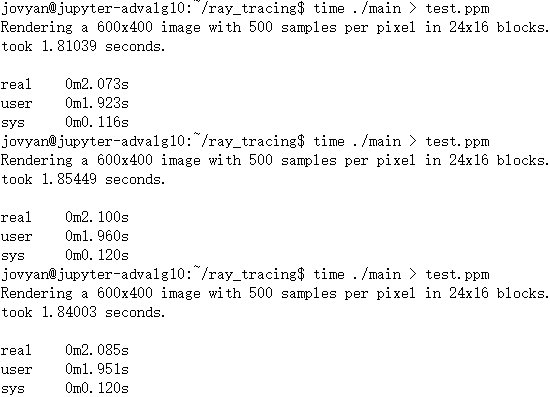
\includegraphics[width=0.8\textwidth]{24x16.png}
    \caption{CUDA with block shape 24x16}
\end{figure}
\begin{figure}[H]
    \centering
    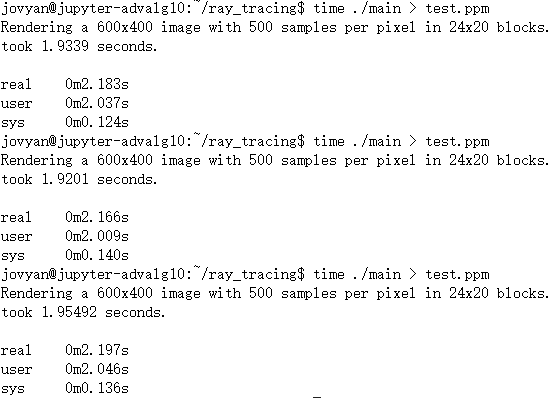
\includegraphics[width=0.8\textwidth]{24x20.png}
    \caption{CUDA with block shape 24x20}
\end{figure}
可以看出加速比在block size为24x16时到达顶峰,接近93,而size过大或过小都没有更优。

上面分析了引入CUDA效率,下面分析正确性。由于随机数因素,难以逐字节对比文件来分析,这里通过直观地对比图片来分析:
\begin{figure}[H]
    \centering
    \includegraphics[width=0.5\textwidth, bb=0 0 20cm 20cm]{test_cpu.bmp}
    \caption{CPU version}
\end{figure}
\begin{figure}[H]
    \centering
    \includegraphics[width=0.5\textwidth, bb=0 0 20cm 20cm]{test.bmp}
    \caption{CUDA version}
\end{figure}
就算有随机因素的情况下,直观上仍找不出两图的差别,基本说明是正确的。
\section{BVH}
获取与最近接触物体的信息,可以通过BVH树搜索优化,来使其由线性复杂度变为对数复杂度。
\subsection{原理简介}
\subsubsection{BVH}
BVH结构如下:
\begin{figure}[H]
    \centering
    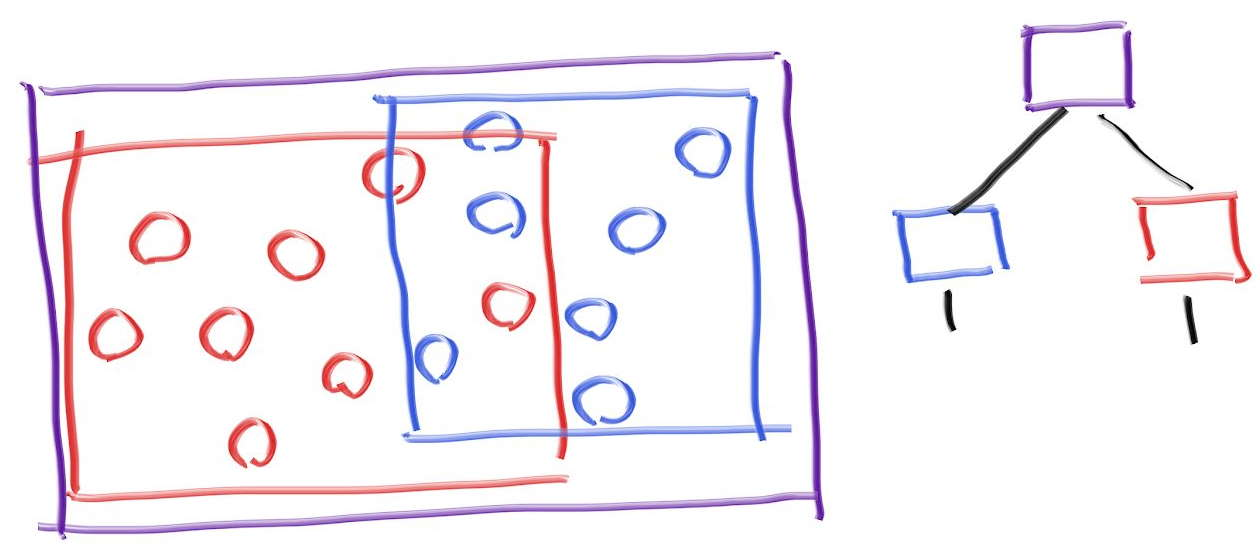
\includegraphics[width=0.8\textwidth]{bvh.jpg}
    \caption{Bounding volume hierarchy}
\end{figure}
圆形是物体即叶子节点,方框是非叶子节点。每个父节点有两个子节点,图形上父节点是包含两个子节点的大框。这样假设物体数量为$N$,如果就能构造出比较平衡的二叉树(即划分左右节点比较均衡),
那它的树高最好可以达到$\log(N)$。而找最近接触物体的伪代码如下:
\begin{lstlisting}
if (hits purple)
    hit0 = hits blue enclosed objects
    if (hit0)
        return true and info of closer hit
    hit1 = hits red enclosed objects
    if (hit1)
        return true and info of closer hit
return false
\end{lstlisting}
由于可以通过hits purple和hit0来提前结束搜索,令其只需遍历一条根到叶子的路径,因而击中物体的情况下最好时间复杂度是$O(\log(N))$。而也有可能击中了全部框体但是却只击中了二叉树中最后
一个物体,但就算是这种最坏的情况,由于二叉树一共$2N-1$个节点,其时间复杂度也是$O(N)$。因而如果能构造出一个比较平衡的二叉树其时间复杂度上将线性优化成了对数。
\subsubsection{AABB}
上述所提到的$O(N)$最坏情况是难以避免的。如果要构造出完全没缝隙的框体,这样会增加hits purple的判断复杂度。考虑两个完全不相交的球,没缝隙的框体是两块球空间的并集,而判断hits purple
则还是只能分别判断是否击中两个球,这样效率只能更低。因此换句话说,构造一个简单的框体是很重要的。这里使用Axis-Aligned Bounding Boxes,其实际上是用与轴平行的线划分方形空间。其计算
hits purple是很简单的,只需看该空间的所有维度的区间在光线上的投影是否重叠:
\begin{figure}[H]
    \centering
    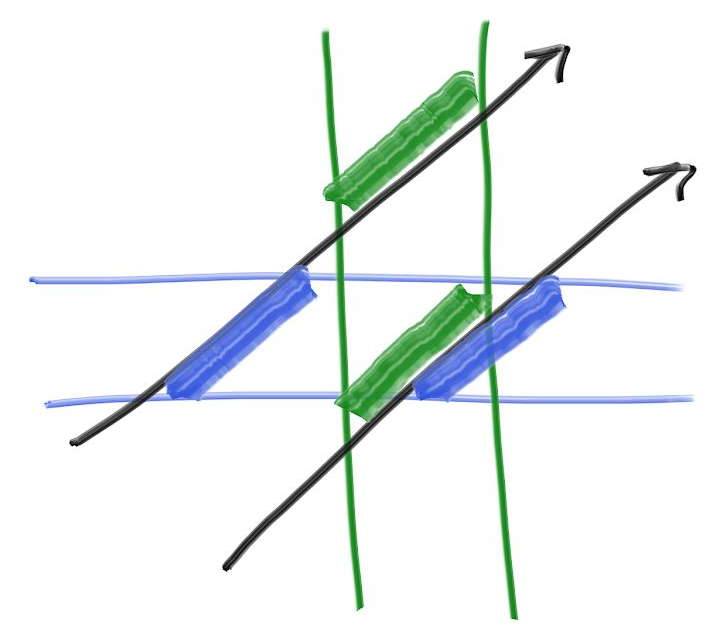
\includegraphics[width=0.8\textwidth]{overlap.jpg}
    \caption{Ray-slab t-interval overlap}
\end{figure}
上图中,两条黑线表示两束光线,蓝色和绿色分别表示两个维度。两个维度在上面光线的投影不重合,因而上面光线不穿过中间的方形区间;两个维度在下面光线的投影重合,因而下面光线穿过方形区间。
\subsubsection{构建BVH}
另一个问题是要达到对数时间复杂度,还要能够造出比较平衡的BVH树。这里使用的方法是每次划分时,随机取一个维度,在上面排序物体,然后二分令两部分物体数量一样。值得注意的是由于CUDA,排序
算法无法使用STL提供的排序,在这里我使用了thrust库提供的排序。
\subsection{实验}
该部分实验基于Ray Tracing In One Weekend的最终场景,CUDA block形状使用最好的24x16,由于这部分优化和物体数量有关,我设置了不同物体数量,分别为:4大球、4大球484小球、4大球1936小球。
\subsubsection{场景设置}
4大球的场景和CUDA实验相同,后面更多球的场景为了加快渲染时间将num\_samples降到了100。
\subsubsection{更多球数量的实现}
4大球和CUDA实验相同,484小球只是将注释掉的部分恢复,1936小球是将484小球的每1个改成4个重叠的小球这样大量框体无空隙是很能体现BVH优势的。
\subsubsection{结果}
\begin{figure}[H]
    \centering
    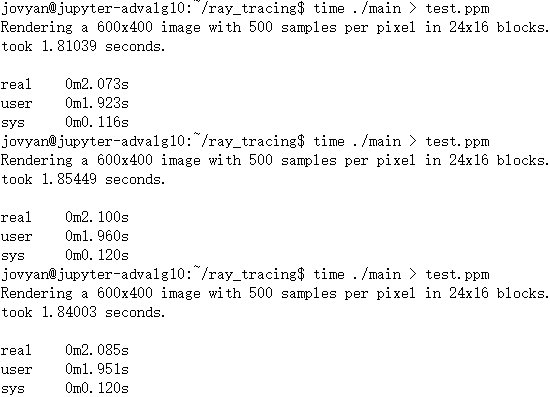
\includegraphics[width=0.8\textwidth]{24x16.png}
    \caption{4 balls without BVH}
\end{figure}
\begin{figure}[H]
    \centering
    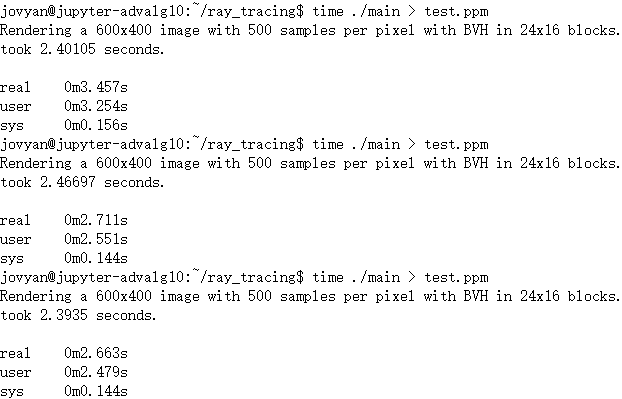
\includegraphics[width=0.8\textwidth]{24x16_bvh.png}
    \caption{4 balls with BVH}
\end{figure}
\begin{figure}[H]
    \centering
    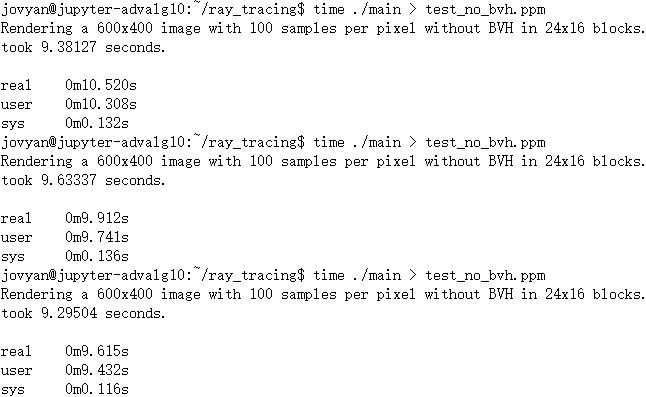
\includegraphics[width=0.8\textwidth]{488_no_bvh.png}
    \caption{488 balls without BVH}
\end{figure}
\begin{figure}[H]
    \centering
    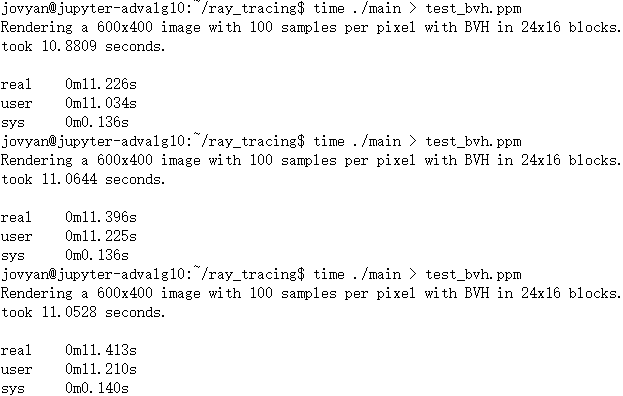
\includegraphics[width=0.8\textwidth]{488_bvh.png}
    \caption{488 balls with BVH}
\end{figure}
\begin{figure}[H]
    \centering
    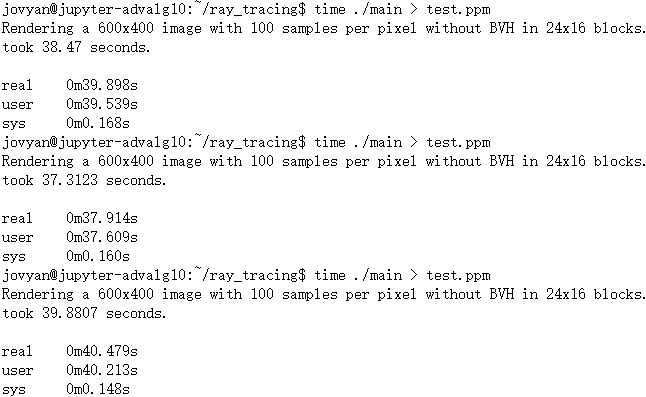
\includegraphics[width=0.8\textwidth]{1940_no_bvh.png}
    \caption{1940 balls without BVH}
\end{figure}
\begin{figure}[H]
    \centering
    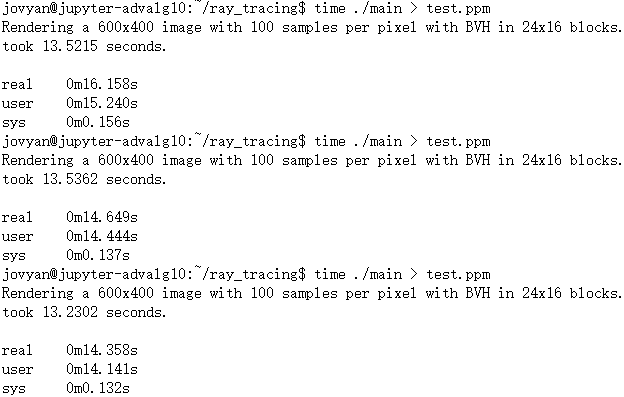
\includegraphics[width=0.8\textwidth]{1940_bvh.png}
    \caption{1940 balls with BVH}
\end{figure}
可以看出在大量物体且缝隙少的场景下,BVH的加速效果明显。而在少量物体场景下,BVH反而慢,因为CUDA执行流复杂任务效果不佳,另外BVH需要大量常数时间。由于BVH的优化只和物体数目有关,在渲染
前可以调小其他参数看开启BVH有无优化再决定是否开启BVH。

下面是正确性的验证,两张图都是从488球的场景下生成的:
\begin{figure}[H]
    \centering
    \includegraphics[width=0.5\textwidth, bb=0 0 20cm 20cm]{test_no_bvh.bmp}
    \caption{image without BVH}
\end{figure}
\begin{figure}[H]
    \centering
    \includegraphics[width=0.5\textwidth, bb=0 0 20cm 20cm]{test_bvh.bmp}
    \caption{image with BVH}
\end{figure}
就算有随机因素的情况下,直观上仍找不出两图的差别,基本说明是正确的。
%\clearpage
%\bibliography{E:/Papers/LiuLab}
%\bibliographystyle{apalike}
\end{document}
%%% Local Variables:
%%% mode: latex
%%% TeX-master: t
%%% End:
